\documentclass[11pt,a4paper]{article}
\usepackage[margin=24mm,headheight=15pt]{geometry}
\usepackage{amsmath,amssymb,mathtools,booktabs,longtable,array,xcolor}
\usepackage{tikz,fancyhdr,microtype,hyperref}
\usetikzlibrary{arrows.meta,positioning}
\definecolor{ink}{HTML}{18334D}
\definecolor{accent}{HTML}{17628F}
\hypersetup{colorlinks=true,linkcolor=accent,urlcolor=accent,pdftitle={Ariadne: a structural type-theoretic reconstruction},pdfauthor={Ariadne source-grounded explanation},bookmarksnumbered=true}
\pagestyle{fancy}\fancyhf{}
\fancyhead[L]{\small Ariadne: structural types and analysis semantics}
\fancyhead[R]{\small 2026-10-20}
\fancyfoot[C]{\thepage}
\setlength{\parskip}{5pt}\setlength{\parindent}{0pt}
\setlength{\tabcolsep}{5pt}\renewcommand{\arraystretch}{1.17}
\emergencystretch=2em
\allowdisplaybreaks
\newcommand{\ty}[1]{\mathsf{#1}}
\newcommand{\rec}[1]{\{\,#1\,\}}
\newcommand{\fin}{\mathcal{P}_{\!f}}
\newcommand{\dom}{\operatorname{dom}}
\newcommand{\lfp}{\operatorname{lfp}}
\newcommand{\out}{\operatorname{Out}}
\newcommand{\incoming}{\operatorname{Incoming}}
\newcommand{\preds}{\operatorname{Preds}}
\newcommand{\gen}{\operatorname{Gen}}
\newcommand{\ent}{\operatorname{Entry}}
\newcommand{\deps}{\operatorname{Deps}}
\newcommand{\local}{\operatorname{local}}
\newcommand{\wf}{\operatorname{WF}}
\newcommand{\code}[1]{\texttt{\detokenize{#1}}}
\newcommand{\llbracket}{[\![}
\newcommand{\rrbracket}{]\!]}
\newcommand{\rulelabel}[1]{\text{\scriptsize\textsc{#1}}}
\newcommand{\source}[2]{\href{run:../../../#1}{\code{#1}}\ --- #2}
\newcommand{\note}[1]{\par\smallskip\noindent\fcolorbox{accent}{accent!4}{\parbox{\dimexpr\linewidth-2\fboxsep-2\fboxrule}{#1}}\par\smallskip}
\newcolumntype{Y}{>{\raggedright\arraybackslash}p{.29\linewidth}}

\begin{document}
\hypersetup{pageanchor=false}
\begin{titlepage}
\color{ink}
\vspace*{16mm}
{\Huge\bfseries Ariadne\par}
\vspace{5mm}
{\LARGE A structural type-theoretic reconstruction\par}
\vspace{8mm}
{\large Immutable evidence, local graphs, possible origins,\par
bounded frame questions and justified claims\par}
\vspace{14mm}
\hrule\vspace{6mm}
\textbf{Source snapshot}\par
\code{184a181a0a09c81bed38c543721bd10970512d89}\par
\textbf{Reading date}: 20 October 2026\par
\textbf{Delivery}: LaTeX source and PDF; explanation only\par
\vspace{8mm}
Ariadne takes one immutable captured snapshot, constructs a finite local
control-flow problem, and computes possible value origins. Its investigation
layers attach questions and evidence to that problem. The useful type-theoretic
view is a family of structured data types refined by validity, coverage and
premise conditions.

\note{This document reconstructs the current implementation in mathematical
notation. It is not a new checked type theory, an implementation plan, or a
replacement for the authoritative analysis-level TLA+ specifications.
Rust and OCaml do not implement the dependent types written here.}
\vfill
\textbf{Reading route}\par
Sections 1--4 connect the explanation to concrete code.
Sections 5--10 reconstruct the analysis machine.
Sections 11--16 give types, judgments and transition rules.
Sections 17--19 map them back to source and explain their limits.
The appendices expand the frame, resolver and completion contracts.
\end{titlepage}
\hypersetup{pageanchor=true}
\tableofcontents
\clearpage

\section{Purpose and module boundary}
\label{sec:purpose}
Ariadne's core answers: \emph{given these roots, these admitted instruction
summaries and these bytes, which local edges and possible data origins follow?}
The machine being modeled is the \emph{analyzer}; its state is not a recovered
historical CPU state.

The production minidump route has the following ownership chain:
\begin{center}
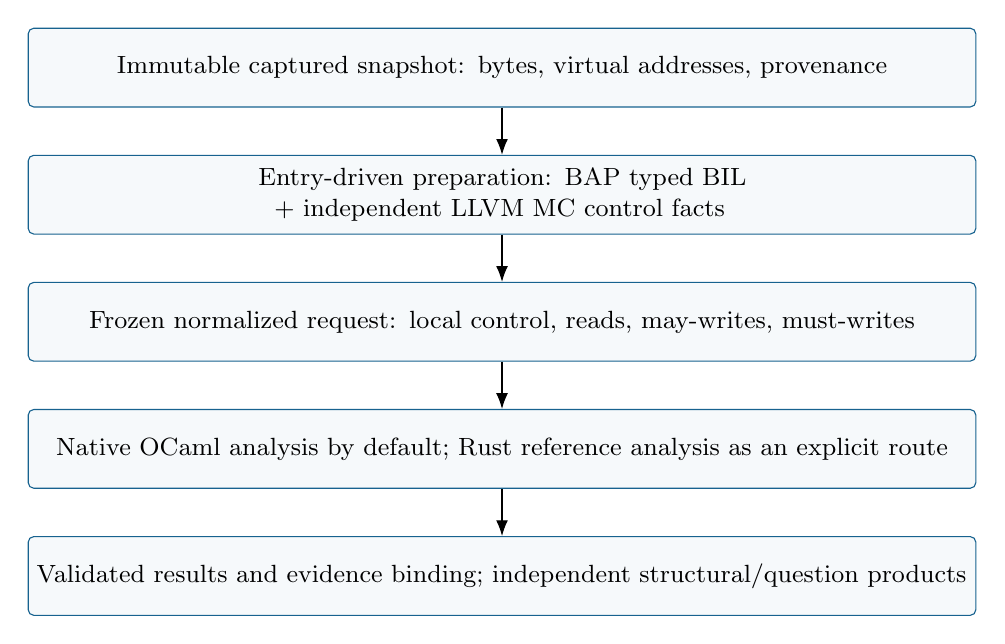
\begin{tikzpicture}[node distance=6mm, every node/.style={font=\small},
 box/.style={draw=accent,rounded corners=2pt,fill=accent!4,text width=11.8cm,align=center,minimum height=10mm},
 >={Latex[length=2mm]}]
\node[box] (a) {Immutable captured snapshot: bytes, virtual addresses, provenance};
\node[box,below=of a] (b) {Entry-driven preparation: BAP typed BIL + independent LLVM MC control facts};
\node[box,below=of b] (c) {Frozen normalized request: local control, reads, may-writes, must-writes};
\node[box,below=of c] (d) {Native OCaml analysis by default; Rust reference analysis as an explicit route};
\node[box,below=of d] (e) {Validated results and evidence binding; independent structural/question products};
\draw[->] (a)--(b);\draw[->] (b)--(c);\draw[->] (c)--(d);\draw[->] (d)--(e);
\end{tikzpicture}
\end{center}
Preparation owns discovery and semantic admission. The core owns recovery,
reaching definitions and slicing over the frozen request. Investigation owns
bound, question-specific claims. Protocol validation connects the native
helper to the Rust host. These responsibilities have different proof boundaries.

The structural frame route branches before full completion: it seals a
recovery prefix, including a drained one, while the core phase is still
\code{Recover}. It can feed frame connections and focused questions without
computing the full reaching-definition table.

\textbf{Scope.} Windows/Linux AMD64 minidumps are implemented; general PE/ELF
image readers and ELF-core readers are deferred. BAP lifting is a pinned trusted
dependency. The independent AMD64 instruction-step model is retired. Supplied
LLVM IR and supplied abstract stateflow are separate analysis paths, not
implicit minidump execution semantics.

\section{Concrete implementation}
\label{sec:concrete}
\begin{longtable}{@{}p{.28\linewidth}p{.66\linewidth}@{}}
\toprule
Carrier or module & What the implementation actually holds or does\\\midrule
\endhead
\code{AnalysisRequest} & Owned snapshot ID, finite address/location sets, entry roots, slice seeds, byte-source sets, successful-decode set and an instruction map total on candidate addresses.\\
\code{Instruction} & Kind, continuation set, known target set, completeness Boolean, uses, must-defs and may-defs. It is an admitted summary, not a numeric CPU state.\\
\code{AnalysisState} & Phase, pending/visited/decoded sets, provenance map, unified typed edge set, obligations, per-site reaching sets and slice.\\
\code{Analyzer} & Owns the validated request and mutable state. Indices, caches and work counters accelerate analysis. Ordinary \code{step} selects the lowest eligible VA.\\
\code{DefinitionSet} & Either an ordered tree or shared sorted definition universe with immutable membership bits. Mutating a dense set creates a private tree representation.\\
Native core & OCaml helper owns production analysis state. Rust checks request/source identity, protocol, pages, result domains and clean completion.\\
\code{CompletedAnalysis} & Private request/state carrier; immutable state is shared through \code{Arc}. It implements sealed \code{AnalysisView}.\\
\code{BoundFrameStructure} & Private owner of a captured frame chain, per-activation bound recovery prefixes, links, maps and diagnostics.\\
\code{BoundFrameConnections} & Owns its structural source and a read-only derived graph assessment.\\
\code{BoundFrameQuestion} & Binds one typed question, admitted evidence, source revision, independent layer assessments and work receipts.\\
\bottomrule
\end{longtable}

\textbf{Mutation and ownership.} The request is validated at construction and
then exposed through shared references. Analysis mutates worklists and facts,
not the request. Later preparation revisions are separate frozen problems,
not a mutation of an already analyzed request. \code{Arc} shares immutable
results; it does not turn one captured snapshot into evidence of concurrent
program execution.

\textbf{Effects and errors.} The pure mathematical core consumes supplied facts.
The surrounding pipeline reads capture files and exchanges bounded messages
with helper processes. Invalid requests and malformed proofs are errors;
unknown targets, unsupported semantics and exhausted question work remain
explicit gaps or layer stops under their respective product contracts.

\section{Concrete invariants and their enforcement}
\label{sec:invariants}
A record can have the correct field types and still violate the analysis
contract. The important obligations are stronger than record shape.

\begin{longtable}{@{}p{.57\linewidth}p{.37\linewidth}@{}}
\toprule Invariant & Principal enforcement\\\midrule\endhead
Snapshot ID and roots are nonempty; instruction map has exactly the candidate domain. & \code{AnalysisRequest::validate}; TLA+ assumptions and address contract.\\
Targets and continuations stay in that domain; uses/may-defs stay in the location domain. & Request validation.\\
Must-defs are a subset of may-defs; continuation/target cardinalities match instruction kind. & Request validation.\\
Only discovered local successors are queued; visited and pending are disjoint. & Construction and transition code; recovery invariants.\\
Call edges remain visible but do not transmit local dataflow into callees. & Explicit edge-kind allowlist, transition equations and conformance controls.\\
Definition origins name a declared entry or a decoded possible writer. & Engine construction, native result checks and model invariants.\\
Slicing begins at the fixed point; done results are dependency-closed. & Phase guards and completion/result validation.\\
Native results bind the exact request, helper and transaction. & Host protocol/session validation; not Rust's field types alone.\\
Captured observations, derived facts and hypotheses retain distinct authority. & Evidence constructors, source/proof validation and report contracts.\\
A true-looking target list also covers every allowed incoming case. & Resolver coverage validation; a list or hash alone is insufficient.\\
\bottomrule
\end{longtable}

Some boundaries remain premises: correct BAP lifting, conservative alias
normalization, the relationship between captured memory and an earlier
instruction, and the distinct identity assigned to each snapshot. Finite model
checks and tests do not prove these premises universally.

\section{Representative execution in the code}
\label{sec:concrete-trace}
Consider one tracked location $x$ and four decoded sites in a single snapshot:
\[
 a_0 \xrightarrow{\mathrm{taken}} a_1 \longrightarrow a_3,
 \qquad
 a_0 \xrightarrow{\mathrm{fallthrough}} a_2 \longrightarrow a_3.
\]
The only root is $a_0$ and the only slice seed is $a_3$.
At $a_1$, a definite write has $\ty{must}=\ty{may}=\{x\}$.
At $a_2$, a possible write has $\ty{must}=\varnothing$, $\ty{may}=\{x\}$.
At $a_3$, the instruction reads $x$ and ends the local scope.
All unmentioned tracked uses and writes are empty.

\code{Analyzer::new} validates the request and queues $a_0$.
\code{step}/\code{visit} discovers both branch edges and then their continuations.
Neither the slice seed nor a crash-time value selects a branch.
After \code{FinishRecovery}, propagation computes:
\begin{align*}
 R(a_0)&=\{\ent(a_0,x)\},\\
 \out(a_1)&=\{\ty{Write}(a_1,x)\},\\
 \out(a_2)&=\{\ent(a_0,x),\ty{Write}(a_2,x)\},\\
 R(a_3)&=\{\ent(a_0,x),\ty{Write}(a_1,x),\ty{Write}(a_2,x)\}.
\end{align*}
\code{FinishDataflow} starts the slice at $\{a_3\}$.
\code{ExpandSlice} adds $a_1,a_2$. Entry origins remain reportable unknown
inputs but are not producer instruction nodes. The final slice is
$\{a_1,a_2,a_3\}$; it excludes $a_0$ because this is a data slice, not a
control-dependency slice. The result says which origins are possible under the
supplied summaries, not which predecessor executed.

\section{First abstraction boundary}
\label{sec:boundary-one}
From concrete storage to the analysis machine we preserve snapshot identity,
semantic VAs, finite request domains, instruction effects, typed edges,
provenance, obligations, phase boundaries, definitions and slice membership.
We erase allocator behavior, \code{BTreeMap} layout, internal indices, cache
contents and membership-word placement. Resource policy is retained as a
separate observable outcome; exact wall-clock behavior is not part of the
unbounded core transition system.

This abstraction deliberately does not invent numeric register values from
uses/may-defs/must-defs. Those sets describe dependencies and writes. A
numeric transfer needs separately admitted BIL semantics or a supplied
stateflow relation.

\section{The minimal abstract machine}
\label{sec:machine}
Fix a valid immutable request $q$. Write $A$ for candidate VAs, $L$ for
locations, $E_0$ for entry roots, $Z$ for slice seeds and $I$ for instruction
summaries. Let $\Delta_q$ be the finite universe of possible definition
identities. An analyzer configuration is
\[
 \Sigma=\langle p,P,V,D,\pi,G,O,R,S\rangle_q.
\]
\begin{center}
\begin{tabular}{@{}ll@{}}\toprule
Component & Meaning\\\midrule
$p$ & Phase: recover, dataflow, slice or done\\
$P,V,D\subseteq A$ & Pending, visited, successfully decoded starts\\
$\pi:A\to\ty{ByteSource}$ & Whole-instruction selected-source provenance\\
$G\subseteq\ty{Edge}(A)$ & All typed edges, including call edges\\
$O\subseteq\ty{Obligation}(A)$ & Explicit unresolved recovery/target obligations\\
$R:A\to\fin(\Delta_q)$ & Possible origins immediately before each instruction\\
$S\subseteq D$ & Backward instruction data slice\\\bottomrule
\end{tabular}
\end{center}
The immutable subscript $q$ is essential: a changed graph or premise set
requires a new bound analysis problem. $R$ is a map of origins, not a map of
machine integers. $G$ may contain edges whose destination is not decoded.
An unavailable destination remains a recovery boundary rather than becoming a
fabricated terminal instruction.

Initialization sets $P=E_0$, $p=\ty{recover}$, every $R(a)=\varnothing$ and all
other set components empty; initially $\pi(a)=\ty{unavailable}$.

\section{Abstract operations}
\label{sec:operations}
The main transformations are:
\begin{align*}
 \ty{validate}&:\ty{RawRequest}\to\ty{ValidRequest}+\ty{InvalidRequest},\\
 \ty{visit}&:\ty{RecoverState}\times A\rightharpoonup\ty{RecoverState},\\
 \ty{propagate}&:\ty{DataflowState}\times D\rightharpoonup\ty{DataflowState},\\
 \ty{expand}&:\ty{SliceState}\rightharpoonup\ty{SliceState},\\
 \ty{finishBounded}&:\ty{Analyzer}\times\ty{Limits}
          \to\ty{CompletedResult}+\ty{CompletionError}.
\end{align*}
A partial operation is enabled only under the relevant phase and work guard.
Native completion additionally crosses transport/validation operations; a
successful helper response is not yet an admitted public result.

Preparation has a different operation:
\[
 \ty{prepare}:\ty{Snapshot}\times\ty{Query}\times\ty{Policy}
 \to \ty{FrozenRequestWithEvidence}+\ty{PreparationError}.
\]
It may discover candidate starts and propose guarded/target refinements before
freezing the final request. That earlier discovery does not replace the core's
subsequent recovery pass.

\section{Reachability and invariants}
\label{sec:reachable}
Representable records strictly exceed states reachable from initialization.
For example, a public \code{AnalysisState} record can be assembled with phase
\code{Done} and inconsistent reaching sets. Field types allow it; a completed
analysis constructor must not admit it.

For valid reachable core states:
\begin{align*}
 P\cap V&=\varnothing,& D&\subseteq V\subseteq A,\\
 P\cup V&=E_0\cup\{e.\ty{dst}\mid e\in G,\local(e)\},\\
 G&=\bigcup_{a\in D}\ty{InstructionEdges}(I(a)),\\
 p\ne\ty{recover}&\Longrightarrow P=\varnothing.
\end{align*}
Moreover $R(a)=\varnothing$ for undecoded $a$; decoded rows contain only valid
entry/writer identities. In slice/done phases all reaching equations are at
the fixed point. At done the slice contains decoded seeds and is closed under
its data producers.

These are reconstructed semantic refinements. TLA+ names the principal
checks \code{TypeOK}, \code{RecoveryInvariant}, \code{DefinitionInvariant} and
\code{ResultInvariant}. Their finite checking and Rust/native conformance are
separate evidence, not a proof that every concrete state transition refines
this presentation.

\section{Abstract execution trace}
\label{sec:abstract-trace}
For the diamond of Section~\ref{sec:concrete-trace}, the permitted sequence has
the shape
\begin{align*}
 \Sigma_0&\xrightarrow{\ty{Visit}(a_0)}\Sigma_1
 \xrightarrow{\ty{Visit}(a_1)}\Sigma_2
 \xrightarrow{\ty{Visit}(a_2)}\Sigma_3
 \xrightarrow{\ty{Visit}(a_3)}\Sigma_4,\\
 \Sigma_4&\xrightarrow{\ty{FinishRecovery}}\Sigma_5
 \xrightarrow{\ty{Propagate}^{*}}\Sigma_6
 \xrightarrow{\ty{FinishDataflow}}\Sigma_7,\\
 \Sigma_7&\xrightarrow{\ty{ExpandSlice}}\Sigma_8
 \xrightarrow{\ty{FinishSlice}}\Sigma_9.
\end{align*}
The star denotes finitely many enabled propagation actions. The specification
allows different eligible-site orders. Ordinary Rust replay chooses its fixed
lowest-VA order; completion-only reverse postorder changes work order while
preserving the intended final fixed point. Equal final states do not imply
equal intermediate replay traces.

If recovery also reaches an unavailable $a_4$, its incoming edge and
$\ty{Unavailable}(a_4)$ obligation survive into $\Sigma_9$.
Done then means the algorithm completed its admitted finite problem; it does
not erase that gap.

\section{Second abstraction boundary}
\label{sec:boundary-two}
The formal presentation below replaces the machine's raw record shape with
structural records, variants and semantic refinements. It preserves all
components needed for the equations and judgments. It erases concrete Rust and
OCaml constructors, message framing, cache invalidation mechanics, numeric
counter encodings and serialization syntax.

We index types by a snapshot, request or activation where those identities
matter. This is an explanatory strengthening of the type notation. The actual
code often stores these indices as strings/integers and checks compatibility
at runtime. There is no claim that Rust statically proves the indices equal.

\section{Abstract syntax and structural types}
\label{sec:types}
\subsection{The notation and its limits}
We use an extensional structural calculus:
\[
 \tau::=\ty{Bool}\mid\ty{Word}_{64}\mid\ty{String}
 \mid\rec{\ell_i:\tau_i}_{i\in J}
 \mid\langle k_i:\tau_i\rangle_{i\in J}
 \mid\fin(\tau)\mid(\tau\to\sigma)
 \mid\{x:\tau\mid\phi(x)\}.
\]
Records give named fields; variants give tagged alternatives. $\fin(\tau)$
is the type of finite sets. $\{x:\tau\mid\phi\}$ is a semantic refinement,
not a statement that an arbitrary host-language record proves $\phi$.

For immutable observations, record width subtyping forgets extra fields:
\[
 \frac{J\subseteq K\qquad\forall j\in J.\;\tau_j<:\sigma_j}
 {\rec{\ell_k:\tau_k}_{k\in K}<:\rec{\ell_j:\sigma_j}_{j\in J}}
 \;\rulelabel{Record}.
\]
This permits using a richer evidence record where a smaller read-only view is
required. It does not permit strengthening an unknown fact, dropping its
premises, or assigning mutable Rust records new subtype relationships.
A view that forgets premise fields does not gain the authority to publish
an unconditional claim; publication still crosses the owning validator.
General subtyping notation follows Pfenning's lecture notes; the Ariadne
instantiations here are our reconstruction.\footnote{Frank Pfenning,
\emph{Lecture Notes on Subtyping}, 15-312, 2003:
\url{https://www.cs.cmu.edu/~fp/courses/15312-f03/handouts/16-subtyping.pdf}.}

\subsection{Identity and instruction structure}
Let $s:\ty{SnapshotId}$ be nonempty and $A_s\subseteq\ty{Word}_{64}$.
\begin{align*}
 \ty{Addr}(s)&\equiv\rec{\ty{snapshot}:\{s\},\ty{va}:A_s},\\
 \ty{Loc}(q)&\equiv L_q,\\
 \ty{Def}(q)&\equiv\rec{\ty{loc}:L_q,\ty{site}:A_q,
                  \ty{origin}:\ty{Entry}+\ty{Instruction}},\\
 \ty{Edge}(q)&\equiv\rec{\ty{src}:A_q,\ty{dst}:A_q,\ty{kind}:\ty{EdgeKind}}.
\end{align*}
The actual core stores bare VAs inside a request carrying one snapshot ID.
The indexed address notation makes that implicit common context visible.
A file offset and a graph node ID are different semantic types even if all
three use integers in an implementation.

\[
\begin{aligned}
 \ty{Insn}(A,L)\equiv\rec{
  &\ty{kind}:\ty{Ordinary}+\ty{Conditional}+\ty{Jump}+\ty{Indirect}\\[-2pt]
  &\hspace{18mm}+\ty{Call}+\ty{Return}+\ty{Stop},\\
  &\ty{fall}:\fin(A),\ \ty{targets}:\fin(A),\ \ty{complete}:\ty{Bool},\\
  &\ty{uses}:\fin(L),\ \ty{must}:\fin(L),\ \ty{may}:\fin(L)}.
\end{aligned}
\]
This is close to the concrete record. Its cross-field constraints are given
by well-formedness, rather than encoded as distinct Rust constructors.

\subsection{A request is a refined record}
\[
\begin{aligned}
\ty{RawRequest}\equiv\rec{
 &\ty{snapshot}:\ty{String},\ A:\fin(\ty{Word}_{64}),\ L:\fin(\ty{String}),\\
 &E_0:\fin(A),\ Z:\fin(A),\ \ty{input}:\ty{Binary}+\ty{Dump},\\
 &C:\fin(A),\ F:\fin(A),\ T:\fin(A),\ D_0:\fin(A),\\
 &I:A\to\ty{Insn}(A,L)}.
\end{aligned}
\]
Here $C,F,T,D_0$ mean captured, file-backed, trusted fallback and decodable.
The display uses dependent fields as shorthand; the raw Rust representation
uses unrestricted sets/maps before validation.
\[
 \ty{ValidRequest}\equiv\{q:\ty{RawRequest}\mid\wf(q)\}.
\]
The semantic domain is refined. The real \code{AnalysisRequest} type itself
still admits invalid defaults; \code{Analyzer::new} checks them.

\section{Bindings and scopes}
\label{sec:bindings}
Ariadne's core does not resolve source-language lexical names. A location
string is an already normalized storage/dependency identifier. Architectural
aliases such as EAX/RAX or vector subviews must have been projected into
compatible tracked locations by the effects layer.

Entry definitions are \emph{scope-qualified unknown inputs}:
\[
 \ent(a,\ell)=(\ell,a,\ty{Entry}),\qquad
 \ty{Write}(a,\ell)=(\ell,a,\ty{Instruction}).
\]
The tag prevents a write at an entry VA from being mistaken for the entry
input at that VA. Different entry roots receive different entry identities.

Frames add a second scope:
\[
 \ty{Node}(s,\alpha)=\rec{\ty{activation}:\alpha,\ty{va}:\ty{Word}_{64}}.
\]
The implemented node is \code{(frame, site)} inside a bound captured chain;
$s,\alpha$ are its implicit owning context. Two recursive activations with
the same instruction VA are different nodes. One static node may still have
many loop visits. A bounded model-prefix occurrence identifies a modeled
visit, not a recovered historical iteration number.

\section{Judgment forms}
\label{sec:judgments}
Every judgment used below has a specific scope:
\begin{longtable}{@{}p{.39\linewidth}p{.55\linewidth}@{}}
\toprule Judgment & Meaning\\\midrule\endhead
$\Gamma\vdash v:\tau$ & The mathematical value has structural/refinement type $\tau$ under declared context $\Gamma$.\\
$\Gamma\vdash q\;\ty{ok}$ & The normalized request satisfies its input contract.\\
$q\vdash\Sigma\;\ty{valid}$ & Machine shape and phase-sensitive invariants hold.\\
$q\vdash\Sigma\xrightarrow{\alpha}\Sigma'$ & An enabled analyzer action transforms this fixed problem.\\
$\Gamma;\Pi\vdash c\;\ty{admitted}$ & Claim $c$ has passed its owning validator under premises $\Pi$ and exact bound source.\\
$\Gamma;\Pi\vdash\rho\;\ty{covers}(a)$ & A checked resolver receipt covers the allowed incoming cases at dispatch $a$ for its bound graph epoch.\\
\bottomrule
\end{longtable}
$\Gamma$ is a mathematical context of identities, domains and admitted
contracts. It is not a new runtime module named Gamma. $\Pi$ records semantic
premises/hypotheses. The last two judgments summarize several real validation
operations; they are not existing proof-assistant theorem names.

\section{Statics: validity and permission to make a claim}
\label{sec:statics}
\subsection{Request well-formedness}
The following schema summarizes \code{AnalysisRequest::validate}.
First define the per-instruction refinement:
\[
\begin{aligned}
\ty{InsnOK}_{A,L}(i)\equiv{}&
 i.\ty{must}\subseteq i.\ty{may}\subseteq L
 \ \land\ i.\ty{uses}\subseteq L\\
 &\land\ i.\ty{fall}\subseteq A\ \land\ i.\ty{targets}\subseteq A
 \ \land\ \ty{Shape}(i).
\end{aligned}
\]
Then the request rule is
\[
\frac{
 \begin{gathered}
 s\ne\epsilon\quad A\ne\varnothing\quad E_0\ne\varnothing\\
 E_0,Z,C,F,D_0\subseteq A\quad T\subseteq F\quad\dom(I)=A\\
 \forall a\in A.\ \ty{InsnOK}_{A,L}(I(a))
 \end{gathered}}
 {\Gamma\vdash q\;\ty{ok}}
 \;\rulelabel{Request}.
\]
$\ty{Shape}$ requires exactly one continuation for ordinary, conditional and
call instructions; none for other kinds. Ordinary/return/stop have no targets;
conditional/direct jump have exactly one target; indirect/call allow finite
supplied target sets. Empty $L$ and $Z$ are legal.

These rules check the consistency of a supplied semantic summary. They do not
prove it matches machine bytes or hardware behavior.

\subsection{Admission has more premises than shape}
A schematic target-completion rule is
\[
\frac{
 \begin{gathered}
 \ty{SourceBound}(\rho,s,e)\quad\ty{ReplayValid}(\rho)\\
 \Gamma;\Pi\vdash\rho\;\ty{covers}(a)\quad
 \ty{Targets}(\rho)=I(a).\ty{targets}
 \end{gathered}}
 {\Gamma;\Pi\vdash I(a).\ty{complete}=\ty{true}\;\ty{admitted}}
 \;\rulelabel{Target-Coverage}.
\]
$e$ is the candidate graph epoch. This rule is deliberately stronger than
``a supported table expression was recognized.'' Recognizing a pattern
permits an attempt; admitting completeness requires covered entrances,
transfers, table data and successors. The core itself trusts the supplied
\code{complete} flag; the production preparation/admission boundary owns the
meaning of that flag.

Likewise a well-shaped hypothesis is not an observation. Conditional normal
selection can be described as
\[
 \Gamma;\Pi\cup\{h:\ty{AlignedAt}(s,\alpha,a,16)\}
 \vdash\ty{NormalContinuation}(a)\;\ty{conditional}.
\]
It must retain $h$ and the baseline unknown alignment verdict. It supplies no
observed RSP and no earlier executed branch.

\section{Dynamics: recovery, fixed point and slice}
\label{sec:dynamics}
\subsection{Selected bytes and recovered control}
For dump input, whole-instruction source selection is
\[
 \ty{Source}_q(a)=
 \begin{cases}
 \ty{Captured},&a\in C,\\
 \ty{File},&a\notin C\land a\in T,\\
 \ty{Unavailable},&\text{otherwise}.
 \end{cases}
\]
For binary input use file bytes only when $a\in F$. Production minidump input
is capture-only; the generic core's fallback contract does not authorize that
reader to fill a hole. A captured decode failure never retries with file bytes.
Let $\ty{CanDecode}(a)$ mean a selected source is available and $a\in D_0$.

For a successful visit, let $G_a$ be all instruction edges, $O_a$ its target
obligations and $\ty{succ}_{loc}(a)$ its local successors. Then
\[
\frac{p=\ty{recover}\quad a\in P\quad\ty{CanDecode}(a)}
 {\langle p,P,V,D,\pi,G,O,R,S\rangle_q
  \xrightarrow{\ty{Visit}(a)}\Sigma'}
 \;\rulelabel{Visit-OK},
\]
where
\begin{align*}
 V'&=V\cup\{a\},& D'&=D\cup\{a\},&
 P'&=(P\cup\ty{succ}_{loc}(a))\setminus V',\\
 G'&=G\cup G_a,& O'&=O\cup O_a,&
 \pi'&=\pi[a\mapsto\ty{Source}_q(a)].
\end{align*}
Unmentioned fields do not change. A failed visit removes $a$ from $P$, marks
it visited and adds unavailable/decode-failed; it adds no decoded node or
fabricated effects. Incoming edges to that failed endpoint remain.

\begin{center}
\begin{tabular}{@{}ll@{}}\toprule
Summary kind & Edges added by successful recovery\\\midrule
Ordinary & $a\xrightarrow{next}b$\\
Conditional & $a\xrightarrow{taken}t$ and $a\xrightarrow{fallthrough}b$\\
Jump & $a\xrightarrow{jump}t$\\
Indirect & $a\xrightarrow{indirect}t$ for every supplied $t$\\
Call & $a\xrightarrow{call}f$ for each callee; $a\xrightarrow{summary}b$\\
Return / stop & No local continuation\\\bottomrule
\end{tabular}
\end{center}
The local edge allowlist is next, taken, fallthrough, jump, indirect, summary.
Call edges are excluded from local discovery and from the dataflow predecessor
relation. Unknown indirect/call targets produce obligations whenever their
summary has $\ty{complete}=\ty{false}$.

\subsection{Reaching definitions are a monotone finite problem}
For decoded $a$, write $R(a)$ for the input origins before $a$:
\begin{align*}
 \gen(a)&=\{\ty{Write}(a,\ell)\mid\ell\in I(a).\ty{may}\},\\
 \out_R(a)&=\{d\in R(a)\mid d.\ty{loc}\notin I(a).\ty{must}\}\cup\gen(a),\\
 \preds(a)&=\{p\in D\mid\exists e\in G.\ \local(e)\land e.\ty{src}=p\land e.\ty{dst}=a\},\\
 \incoming_R(a)&=
 \begin{cases}\{\ent(a,\ell)\mid\ell\in L\},&a\in E_0,\\
 \varnothing,&a\notin E_0
 \end{cases}
 \ \cup\!\bigcup_{p\in\preds(a)}\out_R(p).
\end{align*}
\[
\frac{p=\ty{dataflow}\quad a\in D\quad\incoming_R(a)\nsubseteq R(a)}
 {\Sigma\xrightarrow{\ty{Propagate}(a)}
  \Sigma[R(a)\mapsto R(a)\cup\incoming_R(a)]}
 \;\rulelabel{Propagate}.
\]
Define $F_q(R)(a)=\incoming_R(a)$. The solution reached from bottom is
\[
 R^*=\lfp(F_q)\quad\text{in }\prod_{a\in D}\fin(\Delta_q).
\]
Must-defs can kill old origins in a transfer, but the kill set is fixed, so
$X\subseteq Y$ implies $\out_X(a)\subseteq\out_Y(a)$.
May-defs alone add alternatives and preserve old ones. Cycles are handled by
monotone growth in a finite lattice, not by enumerating loop executions.

\subsection{Phase boundaries and the backward closure}
\[
\frac{p=\ty{recover}\quad P=\varnothing}
 {\Sigma\xrightarrow{\ty{FinishRecovery}}\Sigma[p\mapsto\ty{dataflow}]},
\qquad
\frac{p=\ty{dataflow}\quad R=F_q(R)}
 {\Sigma\xrightarrow{\ty{FinishDataflow}}
  \Sigma[p\mapsto\ty{slice},S\mapsto Z\cap D]}.
\]
For sliced instruction $a$,
\begin{align*}
 \deps_R(a)&=\{d\in R(a)\mid d.\ty{loc}\in I(a).\ty{uses}
                     \land d.\ty{origin}=\ty{Instruction}\},\\
 H_R(S)&=S\cup\{d.\ty{site}\mid a\in S,\ d\in\deps_R(a)\}.
\end{align*}
Expand while $H_R(S)\ne S$. If $H_R(S)=S$, change phase from slice to done.
The resulting slice includes dependencies of \emph{all uses} of every included
instruction; it need not be a minimal dependency set for one output operand.
The branch instruction in our diamond is therefore not automatically included.

\section{Errors, unknowns and partial results}
\label{sec:errors}
The following sum makes the conceptual differences explicit:
\[
 \ty{Outcome}=\ty{Rejected}(\ty{Error})
 +\ty{Stopped}(\ty{LayerReceipt})
 +\ty{Admitted}(\ty{ScopedProduct}).
\]
This is a semantic organization, not one existing public Rust enum. Each API
has its own result type and admission rules.

\begin{itemize}
\item \textbf{Invalid input or forged evidence}: refuse admission. Exhaustion
must not hide malformed identity, schema or proof data.
\item \textbf{Completed core with obligations}: valid completed partial
analysis. The equations are solved on the recovered graph and the gaps survive.
\item \textbf{Bounded core completion failure}: \code{finish_bounded} returns
\code{CompletionError}; it does not publish a stopped prefix as completed.
\item \textbf{Structural prefix}: an independently valid product even without
dataflow. It is not a disguised completed core result.
\item \textbf{Question or connection work stop}: retain admitted facts and
layer-specific unknowns/receipts. A stopped search cannot justify absence.
\item \textbf{Verifier exhaustion}: refuse a trusted result rather than
accepting unverified producer claims.
\end{itemize}
The implemented core predicate is exactly
\[
 \ty{scopeClosed}(r)\equiv
 (r.\ty{phase}=\ty{Done})\land(r.\ty{obligations}=\varnothing).
\]
It is relative to the normalized request and traversal policy. Missing seeds
are reported separately as $Z\setminus D$. Scope closure implies neither all
real paths nor complete callee execution nor recovery of execution history.

\section{Implementation correspondence}
\label{sec:correspondence}
\begin{longtable}{@{}p{.28\linewidth}p{.66\linewidth}@{}}
\toprule Formal construct & Concrete owner or source symbol\\\midrule\endhead
$\ty{Insn}$, $\ty{ValidRequest}$ & \code{src/model.rs}: \code{Instruction}, \code{AnalysisRequest::validate}.\\
$\Sigma$, $\ty{Visit}$, phase steps & \code{Specs/Ariadne.tla}: \code{Init}, \code{Visit}, \code{Next}; \code{src/engine.rs}: \code{Analyzer::step}, \code{visit}.\\
$F_q$, $H_R$ & \code{Specs/Ariadne.tla}: \code{Out}, \code{Incoming}, \code{Dependencies}; Rust engine and native \code{recovery.ml}.\\
Compact fixed-point storage & \code{src/completion.rs}, \code{src/definition_set.rs}, native \code{dense_completion.ml}.\\
Transport admission & \code{src/bap/core_protocol.rs}, \code{core_session.rs}, \code{core_adapter.rs}.\\
Snapshot reads & \code{src/input/address_space.rs}: \code{ByteRead}, \code{ReadStop}; \code{materialize.rs}: preparation.\\
$\ty{covers}$ judgment & \code{src/bap/target_resolution.rs}; private \code{target_resolution/loop_closure.rs}; \code{guard_admission.rs}; combined materialization.\\
Conditional alignment & \code{src/bap/alignment_hypothesis.rs}; \code{Specs/AriadneAlignmentHypothesis.tla}.\\
Bound recovery and frame structure & \code{src/recovery.rs}, \code{src/investigation/frame_structure.rs}; \code{Specs/AriadneFrameStructure.tla}.\\
Corridor and SCC & \code{src/investigation/frame_connections.rs}; \code{Specs/AriadneFrameConnections.tla}.\\
Typed question and values & \code{src/investigation/frame_question/}; \code{memory_refinement.rs}; \code{backward_values.rs}.\\
Completed read-only view & \code{src/analysis_view.rs}: sealed \code{AnalysisView}, private \code{CompletedAnalysis}.\\
Separate stateflow / IR & \code{src/machine_state.rs}, \code{src/llvm_ir.rs}; their separate TLA+ models.\\
\bottomrule
\end{longtable}
The core transition equations closely correspond to the specification.
The admission, coverage and indexed claim rules are higher-level summaries
of multiple validators. The paper's dependent indices and width-subtyping
rule are explanatory constructs, not host-language declarations.

\section{Final abstraction boundary}
\label{sec:boundary-three}
This reconstruction ignores concrete instruction encodings, full numeric CPU
semantics, OS scheduling, exception-handler execution, allocator layout,
network/filesystem scheduling and timing. The core treats byte selection,
decodability and instruction effects as fixed inputs. Resolver/question layers
recover selected semantics only under their own supported contracts.

Assumptions made visible rather than proved here include: snapshot identity
is meaningful; the admitted lifts have their declared semantics; locations
conservatively account for aliases; a captured-control-memory premise is
appropriate for the selected question; and explicit hypotheses are acceptable
conditions for a conditional result. A content hash binds bytes internally;
it does not authenticate capture provenance or prove historical stability.

\section{Model versus implementation: what the types do not prove}
\label{sec:comparison}
\subsection{Excess representable states}
TLA+ addresses range over nonnegative mathematical integers; the Rust
implementation deliberately restricts them to 64-bit VAs. All sets used by
the analysis request are finite. These representation choices are part of
the correspondence obligation.

Rust aliases such as \code{Address = u64} and \code{Location = String} do not
prevent an accidental file-offset/VA mixup by themselves. A
\code{Default::default()} request has invalid empty fields. Public instruction
records can have contradictory kind/target combinations. A completion flag
can be written without a coverage receipt in raw structures. These facts
explain why construction boundaries and validators matter.

Private completed/bound carriers and a sealed read-only trait restrict ways
external callers can fabricate evidence-bearing objects. They do not turn
all semantic contracts into compiler-checked theorems. In particular,
\code{AnalysisView} also admits an in-progress \code{Analyzer}; consumers must
still enforce the phase they require.

\subsection{Preservation and progress, with their boundaries}
The intended preservation statement is
\[
 q\;\ty{ok}\land q\vdash\Sigma\;\ty{valid}
 \land q\vdash\Sigma\longrightarrow\Sigma'
 \ \Longrightarrow\ q\vdash\Sigma'\;\ty{valid}.
\]
For finite valid core requests under the model's fair scheduling, recovery
visits finitely many starts, dataflow adds finitely many facts and slicing adds
finitely many nodes. Thus the unbounded abstract analyzer terminates. This
argument does not promise a small runtime or prevent concrete resource
exhaustion. It is distinct from termination of the analyzed program.

TLA+ finite scenarios, generated replay, independent oracles and compiled
mutation controls test these obligations on declared corpora. They do not
establish universal Rust/OCaml refinement or hardware-level ISA soundness.
This document adds no machine-checked metatheorem.

\subsection{Which questions are computable here?}
A fixed finite graph's reachability, SCCs and reaching-definition least fixed
point are decidable. Simple-path enumeration is finite but can be enormous;
unbounded loop walks may be infinite. General program reachability can be
undecidable under an unbounded-program model. An exact historical path can
also be underdetermined because one snapshot is compatible with several
histories. These are different reasons for not recovering one unique path.

Current Ariadne addresses them with bounded work, explicit supported semantic
profiles, induction for selected loops, independent layer statuses and
question-relative claims. A positive graph path is structural evidence.
A checked model witness is model-relative evidence. Neither is a recording
of the path actually executed before the dump.

\appendix
\clearpage
\section{Frame products as a family of structural interfaces}
\label{app:frames}
The overall system is best modeled as a family of products, not one Boolean
called complete:
\[
\begin{gathered}
\begin{aligned}
\ty{Product}={}&\ty{CoreDone}+\ty{FrameStructure}+\ty{FrameConnections}\\
 &+\ty{FrameQuestion}+\ty{FramePaths}\\
 &+\ty{SuppliedStateflow}+\ty{SuppliedIR},
\end{aligned}\\[4pt]
\begin{aligned}
\ty{ReportStatus}\equiv\bigl\{
 &\ty{binding}:B,\ \ty{recovery}:R_c,\ \ty{connection}:C_c,\\
 &\ty{question}:Q_c,\ \ty{origins}:O_c,\ \ty{history}:H_c\bigr\}.
\end{aligned}
\end{gathered}
\]
The second record is a semantic summary of independent dimensions, not a
single serialized schema shared by every product.

\subsection{Stage 5.1: publish structure before full dataflow}
A recovery prefix conceptually has type
\[
 \ty{RecoveryPrefix}(q)=
 \{\Sigma:\ty{State}(q)\mid p=\ty{Recover}\land\ty{PrefixValid}(q,\Sigma)\}.
\]
Its stop is drained, work-limited or deadline-limited under the owning
recovery contract. Even a drained prefix stays in Recover: no
\code{FinishRecovery}, dataflow or slicing is credited. A failed or pending
endpoint remains a gap attached to the original edge.

Frame structure binds one such prefix per independently recovered activation.
A captured return address helps identify the active call/continuation under
admitted unwind and byte evidence. It does not identify all prior branch
outcomes or all prior values of volatile registers.

\subsection{Stage 5.2: corridor, SCCs and bounded examples}
The represented route graph contains activation-qualified decoded nodes and
admitted local edges whose endpoints lie in the selected function extents.
Call-only destinations are context. A cross-frame transition uses a validated
active-call link. At an intermediate active-call anchor, the matched edge
enters the child while the summary continuation remains context.

For admitted start $u$ and endpoint $v$, completed graph traversals yield
\[
 F=\ty{Reach}_G(u),\quad
 B=\ty{Reach}_{G^{-1}}(v),\quad
 K=F\cap B.
\]
$K$ is the represented corridor. Strongly connected components summarize
cycles without enumerating their walks. The condensation graph is acyclic.
The iterative SCC implementation and bounded BFS/detour examples operate on
this graph, not on a recovered CPU execution.

Its actual connection verdict is a variant:
\[
\begin{aligned}
\ty{RepresentedConnection}={}&\ty{Found}+\ty{AbsentInRepresentedGraph}\\
 &+\ty{UnknownWorkStopped}+\ty{UnavailableAnchors}.
\end{aligned}
\]
Absence requires completed graph construction and reachability. It remains
absence only in that represented graph. A forward-reachable unresolved jump
outside $K$ may reconnect later, so its frontier must be retained too.
SCC completion, corridor completion and example-search completion are separate
statuses. Requested example count NP is bounded; retained examples do not
establish a total path count.

\subsection{Full frame paths are a separate product}
The frame-path route composes admitted frames and uses typed-edge bounded
DFS with visit/work/step constraints. It can need completed per-frame analyses
and additional compatibility evidence. Its enumeration-exhausted field must
be interpreted together with visit limits, graph gaps and semantic scope.
The existence of a Stage 5.2 route does not by itself close the full frame-path
acceptance gate, prove feasibility or establish execution history.

\section{Resolvers, coverage and loop-aware reasoning}
\label{app:resolvers}
\subsection{A resolver is a checked evidence-producing computation}
A useful semantic interface is
\[
 \ty{resolve}:\ty{BoundSource}\times\ty{DispatchQuestion}\times\ty{Limits}
 \to\ty{CandidateEvidence}+\ty{Unknown}+\ty{Error}.
\]
This is an explanatory interface; current Ariadne has private cooperating
modules and one preparation coordinator, not a generic resolver registry.
The code's pattern recognition is over typed transfer/control structure and
captured-read witnesses, not a claim that an opcode name proves a pattern.
Guard admission, ordinary target evaluation and loop-coverage checking have
related but different responsibilities.

A resolution record contains site, finite targets, a complete flag, ordinary
path receipts, unresolved reasons and optional coverage evidence. The
implemented coverage variant is
\[
 \ty{CoverageEvidence}=\ty{ExistingPrefixTree}(\ty{ReceiptRefs})
 +\ty{InductiveDispatch}(\ty{LoopClosureReceipt}).
\]
Thus loop awareness extends the existing resolver's coverage strategy. It is
not selected as a competing plugin when another pattern also matches.

\subsection{Reading a table gives candidates; coverage gives completeness}
For a captured relative-32 table, the recognized target expression is
schematically
\[
 t=\bigl(b+\operatorname{sext}_{32\to64}(M_s[b+4i])\bigr)\bmod2^{64}.
\]
Here $b$ is a proved base, $i$ is a bounded selector and $M_s$ denotes
source-bound captured control-data bytes under the explicit
\code{FrozenCapturedControlData} premise. Hole/conflict/overflow and unsupported
expression forms remain explicit. Captured bytes do not automatically prove
what a mutable heap location held at an earlier execution point.

Finding one witness gives one admitted candidate. Certifying the full target
set requires all permitted selectors/incoming cases, relevant control
coverage and exact read evidence. A partial list cannot be made complete by
truncating a domain, assuming an unproved predecessor impossible, or setting
a Boolean on the producer side.

\subsection{The implemented loop rule}
For a finite local dispatch region $H$, let $J_n$ be a point assertion and
$\llbracket e\rrbracket$ the supported width-aware transfer. Coverage checks
have the form
\begin{align*}
 \ty{EntranceState}(e)&\subseteq J_{e.\ty{dst}},
       &&\text{every region entrance},\\
 \llbracket e\rrbracket(J_{e.\ty{src}})&\subseteq J_{e.\ty{dst}},
       &&\text{every relevant internal edge},\\
 J_{load}&\models(\ty{base}=b\land\ty{selector}\in D_i),
       &&D_i\text{ finite},\\
 \ty{TargetsFromTable}(b,D_i)&=T_{witnessed}=T_{candidate}.
\end{align*}
The private domain has Top, constants, unsigned intervals and finite word
sets. Unknown selector-byte loads may be fresh on every transition; induction
does not require equal selector values across loop iterations. The reviewed
first scope proves a stable base and dispatch domain, and rejects unsupported
relevant writes, opaque calls and unproved clobbers.

Every required captured table entry must already have an independently
replayable ordinary witness. The loop rule adds coverage for those candidates;
it does not invent loop-only targets. Assertions, region entrances/exits,
source hashes and graph epoch are all bound. A new entrance or changed graph
invalidates affected receipts and forces revalidation.

This proves a local invariant for arbitrarily many finite traversals within
the declared abstraction. It does not prove that the program loop terminates,
that all loops are supported, or that this dump followed one of the witnessed
ordinary paths.

\section{Questions and evidence-indexed claims}
\label{app:questions}
The implemented typed question is either an alternative-consistency question
or a fault-dependency question. An alternative selects an existing typed edge
or dispatch and a masked whole-GPR endpoint condition. Fault dependency selects
a captured fault access and may focus a source-discovered load or writer.
Selectors do not add discovery roots or erase other candidates.

A value fact needs more structure than register name and integer:
\[
\begin{aligned}
\ty{Fact}\simeq\rec{
 &\ty{snapshot}:s,\ \ty{activation}:\alpha,\ \ty{revision}:e,\\
 &\ty{point}:(a,\ty{Before}+\ty{After}),\ \ty{location}:\ell,\ \ty{width}:w,\\
 &\ty{instanceScope}:\iota,\ \ty{profile}:m,\ \ty{premises}:\Pi,
 \ \ty{precision}:\ty{Exact}+\ty{Constrained}+\ty{Unknown}}.
\end{aligned}
\]
This summarizes the binding requirements across several concrete carriers.
Two same-named registers at different points or activations are not
interchangeable facts. Exact information is exact only in its declared model,
point and instance scope. Compatible refinements can narrow an abstract value;
incompatible identities cannot simply be joined into one exact pointer.

The actual question verdict enum is
\[
\begin{aligned}
\ty{QuestionVerdict}={}&\ty{Unknown}+\ty{RefutedUnderModel}\\
 &+\ty{PossibleUnderModel}+\ty{PremiseConflict}.
\end{aligned}
\]
A checked witness supports possible-under-model. Refutation needs the relevant
coverage and supported semantics. A well-formed hypothesis conflicting with
an admitted observation produces premise-conflict; it is not permission to
exclude every writer through logical explosion. Malformed proof data remains
an error rather than a premise conflict.

Fair bounded scheduling services source-frontier resolution, constraints,
scalar propagation and origin collection. Each layer retains its own stop.
Source revisions are immutable and bounded; previously checked facts can be
reused only when their identities and dependencies remain compatible.

For memory, the base candidate set is preserved. Unknown aliasing,
interference and incomplete access/instance coverage prevent blanket writer
exclusions. A displayed focus writer changes presentation, not the universe
of possible origins. A compatible completed callee may contribute its already
validated graph and origins; incomplete caller facts are not promoted to a
completed caller analysis.

Alignment hypotheses are also indexed facts. Assuming an effective address is
16-byte aligned admits a selected MOVAPS normal continuation only conditionally.
Baseline Unknown remains visible. An unaligned execution of that instruction
would take its modeled exception alternative; no actual earlier alignment is
observed merely because the investigator selected normal flow.

\section{Exact compact completion changes representation, not the problem}
\label{app:completion}
At the current source revision, caller S6 uses a shared sorted universe
$U=(d_0,\ldots,d_{m-1})$ with a membership vector $b$ per row. Its abstraction is
\[
 \gamma(U,b)=\{d_i\mid0\le i<m\land b_i=1\}.
\]
Union, kill masks and generation masks operate exactly on this representation.
They do not widen or discard origins. Rust uses 64-bit words; native immediate
storage uses 62-bit words internally. The \code{bitmap/v1} transport has its own
canonical dictionary, membership, binding and physical-budget checks; these
are representation facts rather than new abstract origins.

Completion-only iterative reverse postorder improves propagation scheduling.
Ordinary named-action replay retains its previous schedule. The intended
preservation condition is equality of completed states under the same frozen
request, not equal action-by-action traces for the optimized route.

\begin{center}
\begin{tabular}{@{}lr@{}}\toprule
\code{CompletionLimits} default & Bound\\\midrule
Total charged actions & 1,000,000\\
64-bit membership words per plane & 33,554,432\\
Definition identities & 1,000,000\\
Definition-name bytes & 64 MiB\\
Elapsed time & 600 s\\\bottomrule
\end{tabular}
\end{center}
These are explicit finite policies, not a process-memory guarantee. The solver
owns two membership planes. Already-completed prefixes must still satisfy the
total-action cap. Bounded refusal does not publish completion. The existing
unbounded \code{finish} API retains its reference fallback if compact workspace
policy declines. Native framing and completed-result caps remain separate.

\section{Separate supplied-stateflow and LLVM IR families}
\label{app:separate}
\subsection{Finite abstract stateflow}
The supplied-stateflow model is parameterized by a finite state catalogue
$\mathcal C$ and a relation of typed transitions:
\[
 \ty{Step}\subseteq G\times\mathcal C\times\mathcal C,
 \qquad X:A\to\fin(\mathcal C).
\]
Each abstract state has running/faulted/returned/stopped status and a finite
valuation mapping locations to possible abstract values. Entry states,
effects, terminal transitions and complete-sites assertions are additional
inputs. The stateflow solver propagates supported transitions from admitted
entry facts; it does not generate all these semantics from a minidump.

A structural edge may be feasible under a reached transition, provably
infeasible under complete supplied source semantics, or of unknown feasibility.
The current implementation marks an edge infeasible only at completed
stateflow, when its source is reached and declared complete and the edge has
no feasible transition. Unreached sources are tracked separately.
\emph{All structural edges remain in the structural graph.}

This family has its own request, validation, native/reference solvers and
report schema. Completeness here is completeness of the supplied relation
for the declared model, not hardware completeness or evidence that a
capture-time register value held at an earlier branch.

\subsection{Direct verified LLVM IR}
The IR family takes an already supplied and verified function. Its identity
records the artifact, module and function. Its node identifiers are instruction
and block IDs, not semantic machine VAs. Its normalized structure includes block
terminators and successors, SSA value definitions/uses, phi inputs,
conservative memory predecessors and visible callee targets.

Writing $Z_{IR}$ for instruction seeds, the dependency closure has the form
\[
 S^*_{IR}=\lfp\!\left(
 S\mapsto Z_{IR}\cup S\cup
 \bigcup_{i\in S}
 \bigl(\ty{ValueDefPreds}(i)\cup\ty{MemoryPreds}(i)\bigr)
 \right).
\]
The implementation's \code{dependency_preds} begins with supplied memory
predecessors and adds instruction definitions for used SSA values.
Phi inputs and block-control facts have their own normalized admission
constraints; call-target incompleteness remains an obligation. This is a
separate IR dependency analysis. It does not reconstruct original LLVM IR
from the dump or silently supply missing binary instruction effects.

The separation matters in a structural type presentation: an
$\ty{InstructionId}$ or a supplied catalogue state cannot be substituted for
$\ty{Addr}(s)$ or a captured concrete register merely because their encodings
look compatible. The relevant semantic identity and producer contract differ.

\section{Current evidence and remaining scope}
\label{app:evidence}
The 2026-10-19 caller S6 record is retained evidence bound to its source
capsule, tools, original dump and normalized requests. For the current
\code{184a181} code, its publication receipt confirms that all 980 qualified
runtime/model/test/tool/Cargo inputs are unchanged; later publication deltas
are documentation-only. This explanation reads that record and current source;
it does not rerun the remote qualification.

\begin{center}
\begin{tabular}{@{}lrr@{}}\toprule
Retained original profile & Caller frame 1 & Callee frame 0\\\midrule
Decoded instruction sites & 9,589 & 778\\
Edges & 11,321 & 895\\
Reaching-definition memberships & 141,301,903 & 1,304,602\\
Charged actions & 91,175 & 3,587\\\bottomrule
\end{tabular}
\end{center}
Both saved and raw original requests match, and the completed Rust/native
states agree under the declared original local-normal-flow, empty-seed profile.
The retained record includes row-by-row independent checks, root/features/
Clippy gates, 113 finite model configurations, 330 replay observations and 29
compiled mutation controls. These are scoped observations, not general release
or universal refinement certification.

The original caller-barrier gate is cleared in that profile. Later MOVAPS
alignment, two callee indirect jumps, the separate frame-path F4 gate, broader
large-report/release qualification, executed history/root cause and universal
refinement remain unresolved or separate. Complete caller dataflow can coexist
with incomplete control/evidence elsewhere.

\section{Source map, origin and direct follow-up}
\label{app:sources}
\textbf{Status.} Source-grounded explanatory reconstruction of local revision
\code{184a181}; not a new canonical feature design or proof artifact.
\textbf{Motivation.} Explain the current model through structural types without
conflating data shape, admitted evidence and execution history.
\textbf{Contribution.} The four-level reconstruction, types, judgments and
worked example connect concrete carriers to their scoped meanings.
\textbf{Limits.} Dependent/refinement indices are mathematical notation;
conformance and validation remain separate from universal proof.

The direct origins and next readings are the following inspected sources.
Links target the local checkout relative to this archived PDF; the manifest
records their bytes at the stated revision. A later checkout can change those
files, and PDF-reader policy can restrict launching source links:
\begin{enumerate}
\item \source{Specs/Ariadne.tla}{authoritative normalized core transitions and invariants.}
\item \source{Specs/README.md}{active model ownership and explicit abstraction boundaries.}
\item \source{src/model.rs}{actual records, enums and request validator.}
\item \source{src/engine.rs}{Rust reference state machine and completion entry points.}
\item \source{src/completion.rs}{bounded exact fixed-point completion.}
\item \source{src/definition_set.rs}{shared universe and exact membership semantics.}
\item \source{src/analysis_view.rs}{sealed views and private completed carrier.}
\item \source{docs/Ariadne/architecture.md}{production ownership and separate IR/stateflow routes.}
\item \source{docs/Ariadne/file-reader-design.md}{captured-read, discovery and independent entry contract.}
\item \source{docs/Ariadne/bap-analysis-core-design.md}{native protocol and backend admission boundary.}
\item \source{docs/Ariadne/guarded-target-resolution-design.md}{candidate/final graph layering and loop-coverage contract.}
\item \source{src/bap/target_resolution/loop_closure.rs}{actual coverage variants and assertion receipts.}
\item \source{docs/Ariadne/investigation-design.md}{Stage 5.1, alignment, Stage 5.2 and frame-path distinctions.}
\item \source{docs/Ariadne/frame-question-investigation-design.md}{question identities, evidence, candidate preservation and fair work.}
\item \source{src/investigation/frame_question/model.rs}{actual typed questions, verdicts and policies.}
\item \source{docs/Ariadne/caller-semantic-coverage-design.md}{S6 implementation and its accepted finite profile.}
\item \source{evidence/Ariadne/caller-semantic-coverage/20261019/README.md}{retained source/tool/corpus-bound qualification, not a new run.}
\item \source{docs/Ariadne/semantic-assurance.md}{BAP trust decision and open universal refinement boundary.}
\item \source{ROADMAP.md}{direct successor reading for remaining work and product direction.}
\end{enumerate}

For notation, Pfenning's \href{https://www.cs.cmu.edu/~fp/courses/15312-f03/handouts/16-subtyping.pdf}{subtyping notes}
explain subsumption. Harper's \href{https://www.cs.cmu.edu/~rwh/pfpl/abbrev.pdf}{\emph{Practical Foundations for Programming Languages}, second-edition preview}
provides background on judgments, statics and dynamics. The Ariadne-specific
formulas in this document are independently reconstructed from the sources
above and are not quoted theorems from either text.

The accompanying manifests retain the identity of this explanation:
\begin{itemize}
\item \code{source-manifest.json}: inspected source files and their hashes.
\item \code{render-receipt.json}: PDF, LaTeX source and rendering checks.
\end{itemize}
These records do not refresh the qualification archives or authenticate a capture.
\end{document}
